\documentclass[12pt,a4paper]{scrartcl}		% KOMA-Klassen benutzen!

\usepackage[utf8]{inputenc}			% Zeichensatzkodierung
\usepackage{graphicx}				% Einbinden von Bildern
\usepackage{color}				% Farben wenn es sein muß
\usepackage{amsmath}		
\usepackage{amsfonts}
\usepackage{listings}

\definecolor{codegreen}{rgb}{0,0.6,0}
\definecolor{codegray}{rgb}{0.5,0.5,0.5}
\definecolor{codepurple}{rgb}{0.58,0,0.82}
\definecolor{backcolour}{rgb}{0.95,0.95,0.95}

\lstdefinestyle{mystyle}{
    backgroundcolor=\color{backcolour},   
    commentstyle=\color{codegreen},
    keywordstyle=\color{magenta},
    numberstyle=\tiny\color{codegray},
    stringstyle=\color{codepurple},
    basicstyle=\ttfamily\footnotesize,
    breakatwhitespace=false,         
    breaklines=true,                 
    captionpos=b,                    
    keepspaces=true,                 
    numbers=left,                    
    numbersep=5pt,                  
    showspaces=false,                
    showstringspaces=false,
    showtabs=false,                  
    tabsize=2
}

\lstset{style=mystyle}

\newcommand\svthema{INF264 Project 3}
\newcommand\svperson{Sophie Blum and Benjamin Friedl}
\newcommand\svdatum{30.10.2020}
\newcommand\lvname{Digit recognizer - Report}
\begin{document}

\title{ \svthema}
\author{\textsc{\lvname}}
\date{ \small \textsl{\svperson} --- \svdatum }
\maketitle

\abstract
About the document:
Benajmin developed the classes for the KNN and the SVM model and Sophie developed the CNN model. 
The corresponding reports are also written by that person.

About the code:
We put all classes together in the same file, as we tested our code on google colab. The classes 
could be seperated into different files for better readability.

\section{Candidate Algorithms}
    We wanted to test a variety of different algorithms for this task and therefore decided on three different 
    basic models. We then focussed on evaluating each hyperparameter in a wider range, to get a feeling for the behaviour 
    of each algorithm on our dataset.
    We considered the chosen algorithm the best suited ones for the given classification task.

    \subsection{K-Nearest-Neighbour-Classifier}
        For the K-NN we used the implementation of sklearn and tested the number of neighbours in range(1,8).  
\begin{lstlisting}[language=Python]
    degrees = range(1,8)
    for k in degrees:
        knn = make_pipeline(pca, KNeighborsClassifier(n_neighbors = k))
        knn.fit(X_train, Y_train)
\end{lstlisting}

    \subsection{Support-Vector-Machine-Classifier}
        We chose a Support-Vector-Classifier, using a “one-versus-one”-approach for the multi-class classification. 
        We used the implementation of sklearn. As kernel, we decided to use a polynomial one, testing the degrees in range(1,8). 

\begin{lstlisting}[language=Python]
    degrees = range(1,8)
    for k in degrees:
        svm = make_pipeline(pca, SVC(kernel="poly", degree=k))
        svm.fit(X_train, Y_train)
\end{lstlisting}

    \subsection{CNN}
        A CNN has many hyperparameters that can be tuned. We decided on working with different learning-rates and the number of epochs. We decided 
        on these hyperparameters, as we expect them to have a higher impact on the resulting accuracy as well as the time-performance of the model.
        \subsubsection{Hyperparameters}
            The learning rate has a direct impact on how fast the model can be trained and how accurate the trained weights are in the end.
            A smaller learning rate is good to get more accurate weights, but with the slower rate it also takes more time to compute these.
            A higher learning rate is good to compute the weights fast, but the weights may not be optimal or the training itself is not stable.
            These assumptions are later confirmed by the training and validation results.

\begin{lstlisting}[language=Python]
    learning_rates = [0.01, 0.001, 0.0001, 0.00001]
    for lr in self.learning_rates:
        cnn = self.create_cnn(lr)
        cnn_train = cnn.fit(X_train, Y_train, validation_data=(X_val, Y_val), epochs = 15, verbose=0)
\end{lstlisting}

            We are also using the Adam-optimizer, which is a standard optimizer, that adapts the learning rate during the training. To get the best possible 
            result, we train the model with different starting learning rates.

\begin{lstlisting}[language=Python]
    opt = Adam(learning_rate=lr)
    cnn.compile(optimizer=opt, loss='categorical_crossentropy', metrics=['accuracy'])
\end{lstlisting}

            The number of epochs is an important factor when it comes to overfitting, but also plays a role in the time needed to train the cnn and the 
            resulting accuracy in combination with the learning rate.

            If a very small learning rate is chosen, there are more epochs needed to get the desired result, whereas less epochs are needed with 
            a higher learning rate.
            After a certain amount of epochs, the cnn also starts to overfit to the trainingdata, which can be seen when looking at validation loss and accuracy 
            compared to training accuracy.
            To get the best possible model, we train for 20 epochs and look at the corresponding accuracies and losses after each epoch in the end.

            All other hyperparameters are set on the best-practice standard to not overcomplicate the choosing process. Evaluation a combination of the two 
            chosen hyperparameters already uses a lot of time and adding more values would extend the runtime a lot.

\section{Preprocessing}
    As Convolutional Neural Networks use the data in the form of matrices and the K-Nearest-Neighbour-Classifier as well as the 
    Support-Vector-Machine-Classifier in form of vectors, the pre-processing of the data is different for these models
    \subsection{CNN}
        The input of the CNN can be the images themselves, so that there is no need to do feature-extracting preprocessing steps.
        To feed the data into the CNN, we still need to do some minor preprocessing.
        First the dimensionality of the images needs to be changed. The original shape of each image is (28,28) and gets changed to (28,28,1).
        Each image is now a 28x28 matrix of greyscale values. It is also possible to have colored images. In this case the shape of the input 
        would be (28,28,3).
\begin{lstlisting}[language=Python]
    X_train = X_train.reshape(X_train.shape[0], 28, 28, 1)
    X_test = X_test.reshape(X_test.shape[0], 28, 28, 1)
    X_val = X_val.reshape(X_val.shape[0], 28, 28, 1)
\end{lstlisting}
        In addition, the labels need to be converted to a one-hot-encoding format. Each targetvector is now a vector with 10 rows, indicating 
        each number as the label (1) or not the label (0).
\begin{lstlisting}[language=Python]
    y_data_ohe = []
    for label in y_data:
        ohe_list = [0 for _ in range(10)]
        ohe_list[label[0]] = 1
        y_data_ohe.append(ohe_list)
    y_data_ohe = np.array(y_data_ohe)
\end{lstlisting}

    \subsection{KNN and SVM}
        Every Datapoint describes a 28x28 Pixel big picture and therefore has 784 dimensions. To train a SVM with a polynomial kernel with a 
        higher degree or a K-NN searching for more neighbours is too expensive. Therefore, we applied a Principle Component Analysis on the data. 
        We tested the number of kept dimensions in range(2,20) and calculated the explained variance having those. 

\begin{lstlisting}[language=Python]
    explained_variance = []
    dimensions = range(2,20)
    for i in dimensions:
        pca = PCA(n_components=i)
        pca.fit(X_train)

        explained = 0
        for j in range(1,i):
            explained += pca.explained_variance_[j]
            
        explained_variance.append(explained)
\end{lstlisting}

        We plotted the results, seen in figure \ref{fig::expl_var}.

        \begin{figure}[h]
            \centering
            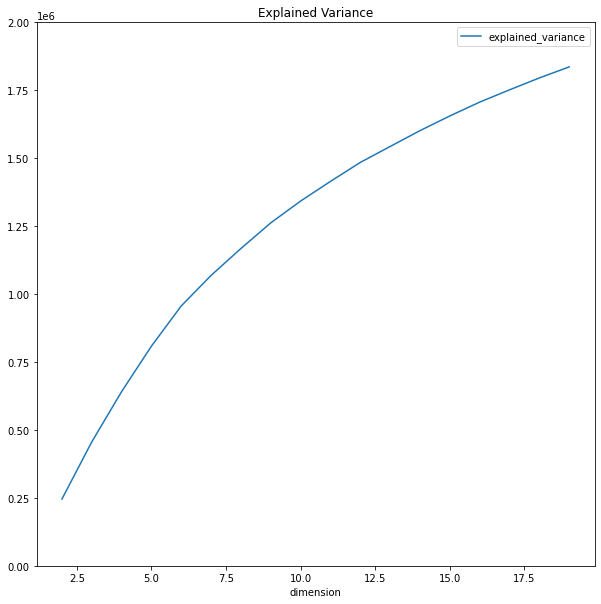
\includegraphics[scale = 0.45]{expl_var.png}
            \caption{Explained variance}
            \label{fig::expl_var}
        \end{figure} 

        We decided to keep 12 dimensions, as the curve starts to flatten there. 
        Additionally, we tried to scale the data before giving it to the PCA. However, the accuracy of the best model on validation-data was 
        ca. 2 \%-2.5\% worse than without using it. This might be due to the fact that we normalised the data without using information about 
        the labels and therefore might have blended them into each other.
        This PCA got built into the models through \texttt{make\_pipeline()} as implemented in sklearn. 

\begin{lstlisting}[language=Python]
    svm = make_pipeline(pca, SVC(kernel="poly", degree=k))
\end{lstlisting}

\section{Performance Measure}
    Generally, the number of datapoints for each label is approximately the same and therefore using accuracy as performance-measure is not susceptible to return a majority-class-classifier. 
    For cnn we also use accuracy as the performance measure, but to select a cnn-model out of all trained cnn-models, we additionally take the validation 
    loss into account. Evaluation the accuracy-loss-ratio gives a good idea of overfitting as well, as the loss starts to grow with an overfitted model and therefore 
    the used measure gets smaller. \\ 
    The accuracies for the SVM’s and K-NN’s are already implemented by sklearn in the function \texttt{score()}.\\
    The accuracies for the cnn are also directly derived through \texttt{history['accuracy']} or \texttt{history['val\_accuracy']}of the cnn model.


\section{Model-selection-scheme}
    We split the given data into training-, validation- and test-data in a ratio of 0.8, 0.1, 0.1 using the function \texttt{train\_test\_split()} as defined in sklearn. 
\begin{lstlisting}[language=Python]
    seed = 414
    X_train, X_val_test, Y_train, Y_val_test = model_selection.train_test_split(X,Y, test_size = 0.2, shuffle=True, random_state=seed)
    seed = 213
    X_val, X_test, Y_val, Y_test = model_selection.train_test_split(X_val_test,Y_val_test, test_size = 0.5, shuffle=True, random_state=seed)
\end{lstlisting}
    Therefore, using only the training-data to fit the models ensures an accurate model whilst having enough validation-data to find a model that is not overfitted. In the end, we choose the model with the highest performance as defined above and use the test-data to estimate the performance in real life. 

\section{Results}
    \subsection{KNN}
        The validation- and training-accuracies are seen in figure \ref{fig::acc_knn}.  
        The best performance is reached for k=5 with an validation-accuracy of 0.95. 

        \begin{figure}[h]
            \centering
            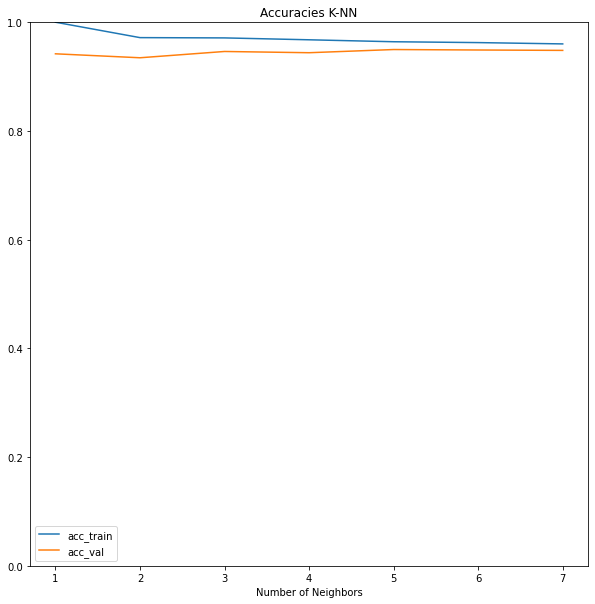
\includegraphics[scale = 0.45]{acc_knn.png}
            \caption{KNN accuracy}
            \label{fig::acc_knn}
        \end{figure} 

    \subsection{SVM}
        The validation- and training-accuracies are seen in figure \ref{fig::acc_svm}
        The best performance is reached for k=3 with a validation-accuracy of 0.9436. After that this model starts to overfit. 

        \begin{figure}[h]
            \centering
            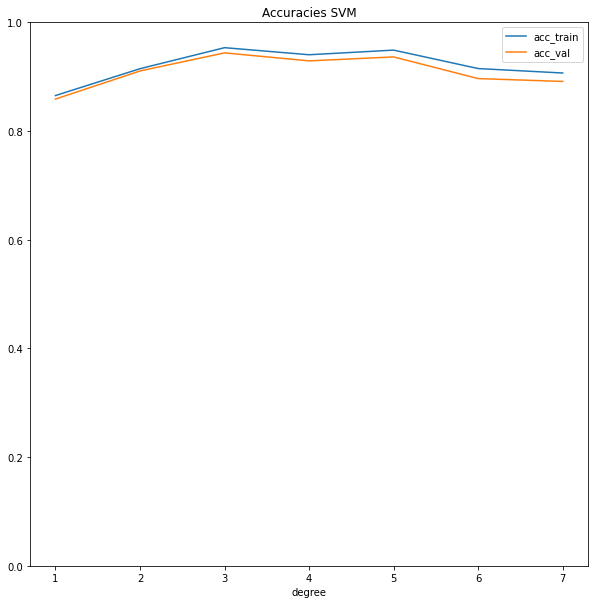
\includegraphics[scale = 0.45]{acc_svm.png}
            \caption{SVM accuracy}
            \label{fig::acc_svm}
        \end{figure} 

    \subsection{CNN}
        The validation- and training-accuracies and -losses are seen in figures 
        \ref{fig::cnn01}, \ref{fig::cnn001}, \ref{fig::cnn0001} and \ref{fig::cnn00001}.
        One can see, that a big learning rate like in figure \ref{fig::cnn01} results in a random behaviour and the model not being 
        trained properly. For the smallest learning rate it is visible, that the accuracy starts to increase more slowly and is way lower 
        in the beginning than with the other learning rates.
        The lower the learning rate, the slower increses the loss as well.\\
        These observations confirm the assumptions we made earlier about learning rates and epochs.

        The combination of these observations can be seen when looking at the accuracy-loss-ratio in figure \ref{fig::acc_loss}.
        For a learning rate of 0.0001 the ratio starts to decrease after 5 epochs, which is due to overfitting. The smaller learning rate does 
        not reach the maximum in the given number of epochs.

        \begin{figure}[h]
            \centering
            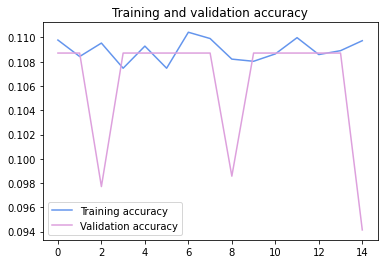
\includegraphics[scale = 0.5]{acc_01.png}
            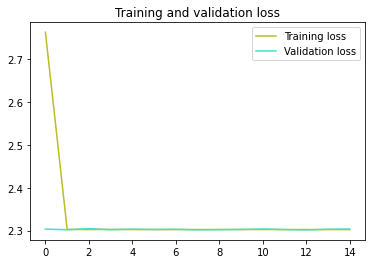
\includegraphics[scale = 0.5]{loss_01.png}
            \caption{Learning rate = 0.01}
            \label{fig::cnn01}
        \end{figure} 
        \begin{figure}[h]
            \centering
            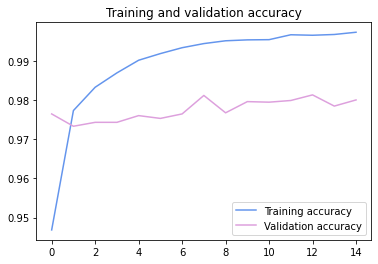
\includegraphics[scale = 0.5]{acc_001.png}
            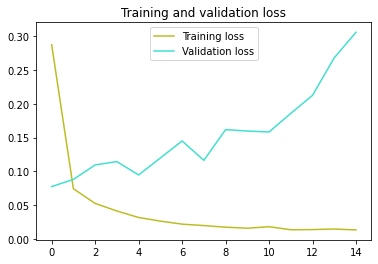
\includegraphics[scale = 0.5]{loss001.png}
            \caption{Learning rate = 0.001}
            \label{fig::cnn001}
        \end{figure} 
        \begin{figure}[h]
            \centering
            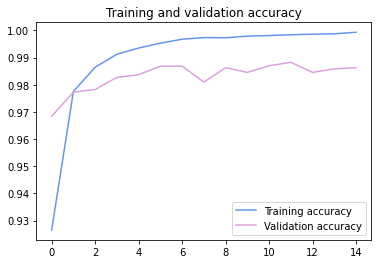
\includegraphics[scale = 0.5]{acc0001.png}
            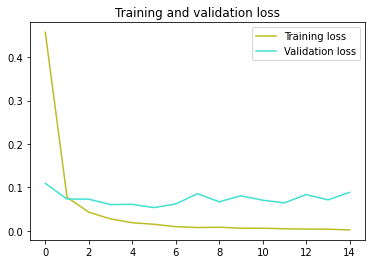
\includegraphics[scale = 0.5]{loss0001.png}
            \caption{Learning rate = 0.0001}
            \label{fig::cnn0001}
        \end{figure} 
        \begin{figure}[h]
            \centering
            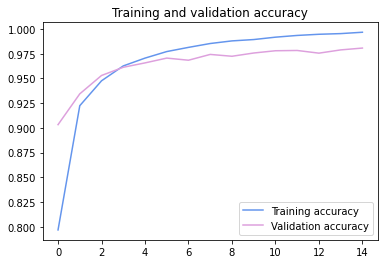
\includegraphics[scale = 0.5]{acc00001.png}
            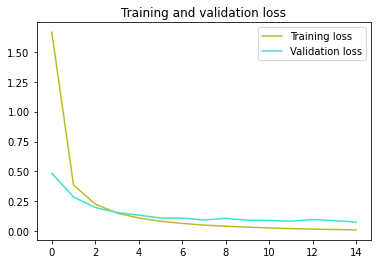
\includegraphics[scale = 0.5]{loss00001.png}
            \caption{Learning rate = 0.00001}
            \label{fig::cnn00001}
        \end{figure} 

        \begin{figure}[h]
            \centering
            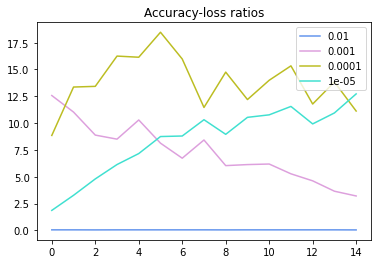
\includegraphics[scale = 1.0]{acc_loss_ratios.png}
            \caption{Accuracy-loss-ratio}
            \label{fig::acc_loss}
        \end{figure}
    
        \subsection{Best model}
            The chosen model with the best accuracy is the Convolutional Neural Network with a learning rate of 0.0001 and 
            5 epochs. This model scores an accuracy of 98.09\% on the test data. Its learning rate is small enough to get accurate rates 
            but also high enough to reach the best accuracy in a reasonable amount of epochs.
            This means, that the model can be trained faster, than a model with a smaller learning rate, although the latter may result 
            in a better accuracy, if trained for a bigger amount of epochs.\\
            As we want our model to be able to be trained faster, we limited the number of epochs to 15 and therefore got a model, that can 
            perform very well in a reasonable amount of time.

\end{document}